\documentclass{article}
\usepackage[utf8]{inputenc}
\usepackage{algpseudocode}
\usepackage{cite}
\usepackage{graphicx}
\linespread{2}
\title{15618 Final Report}
\author{Ziyan Zhang, Xuanyi Li}
\date{May 2022}

\begin{document}

\maketitle

\section{Summary}
We implemented Barnes Hut algorithm for N-Body problem using OpenMP and MPI, and compared the performance among the two parallel versions and the sequential version on PSC machines.

\section{Background}
In physics, the N-body problem is to predict the individual movements of a group of stars and planets that are influenced by each other through gravitational forces. The gravitational forces change the speeds and positions of the objects, and in turn, the positions will change the forces among them. Our goal is that given the initial information about these objects (position, velocity, mass and time), predict its true orbits and trajectory for any future time.

Barnes Hut algorithm consists of two parts that can be parallelized: tree building and force computing. In tree building, it recursively divides the n-bodies into groups and build the tree. In the force computing, it traverses the tree to calculate the forces and update the positions. Both parts could be benefit from the parallelism since the computation for each body is independent of others. We use the pseudocode provided in lecture as a basic idea.

The key data structure in this algorithm is QuadTree where each tree node has four children nodes for topleft, topright, bottomleft, bottomright of the whole graph. 
During tree building, the key operation is inserting that each body will be inserted into the QuadTree recursively until the node contains only one particle. During force computing, the key operation is traversing that each body need to traverse the tree to compute forces. For each iteration, the input of the algorithm is a list of bodies with their position, velocity, and mass while the output is a list of updated bodies based on their interaction in one timestep. Both the tree building part and the force computation part could benefit from parallelization and force computation is more computationally expensive. The force computation depends on the tree construction so we could first finish tree construction in parallel and then work on force computation in parallel.

\section{Approach}

We implemented our methods using C++ in OpenMP and OpenMPI. We targeted machines with large number of cores that can fully utilize the parallelism provided by our implementation such as PSC machines.

The pseudo code for our project is as follows:
\begin{algorithmic}

\For{\texttt{each time step in simulation}}
\State{\texttt{build tree structure}}
\State{\texttt{compute (aggregate mass, center-of-mass) for interior nodes }}
\For{\texttt{each particle}}
\State{\texttt{update position and velocity based on gravitational forces}}
\EndFor
\EndFor

\end{algorithmic}

The QuadTree is hard to distribute to different nodes as in our representation, each node will only store the addresses of their children, instead of storing objects directly. Sharing the whole tree among different nodes would be complicated, so in our MPI implementation the each node builds the tree itself instead of parallely constructing the tree in the OpenMP version. Particles are much easier to distribute to different nodes as they only carry their own position, velocity and mass information. In both implementations, each node/thread will be responsible for computing a chunk of particles and update the information with others.

In the tree construction phase, we first tried to divide the particles uniformly into each thread, but we found that there were too many collisions when merging the tree. So we divide the particles by their positions, which maps to the four children in the QuadTree, and merging the tree will have no conflict as the particles processed by different thread belongs to a different QuadTree.

In the force computation phase, the workload distribution is much easier. The computation of each particle is independent and doesn't affect computation of others, so it can be assigned to any thread/node. Each thread/core will receive an equal number of particles. In the OpenMP implementation, the list of particles is shared among worker threads, so each thread can directly update the particle information. In the MPI implementation, each node has its own address space, so it processes a fixed set of particles, and communicates with each other when every node has finished the computation. To be more specific, we use the AllGather() to collect the updated data.

We start from the pseudo code provided by \cite{pseudo_code}, input files provided by \cite{input}, and visualization code provided by \cite{visualization}.




\section{Experiments and Results}

\subsection{Metrics}
We used execution time as a measurement and compared the speedup between sequential and parallel versions.

\subsection{Setup}
For experiment, we used two input files with about 10K and 30K particles, named Galaxy10K and Galaxy30K, and run for 10 iterations on PSC machines. We measured the tree time for tree construction, force time for force computation and total time (tree time + force time), and compared the speedup on 4, 16, 64 threads/cores with single thread version.

\subsection{Results}
We presented the results of our experiments in Figure~\ref{10k_openmp},\ref{10k_mpi},\ref{30k_openmp},\ref{30k_mpi}. We would analyze our results from three different perspectives. 


\begin{figure}[h!]
  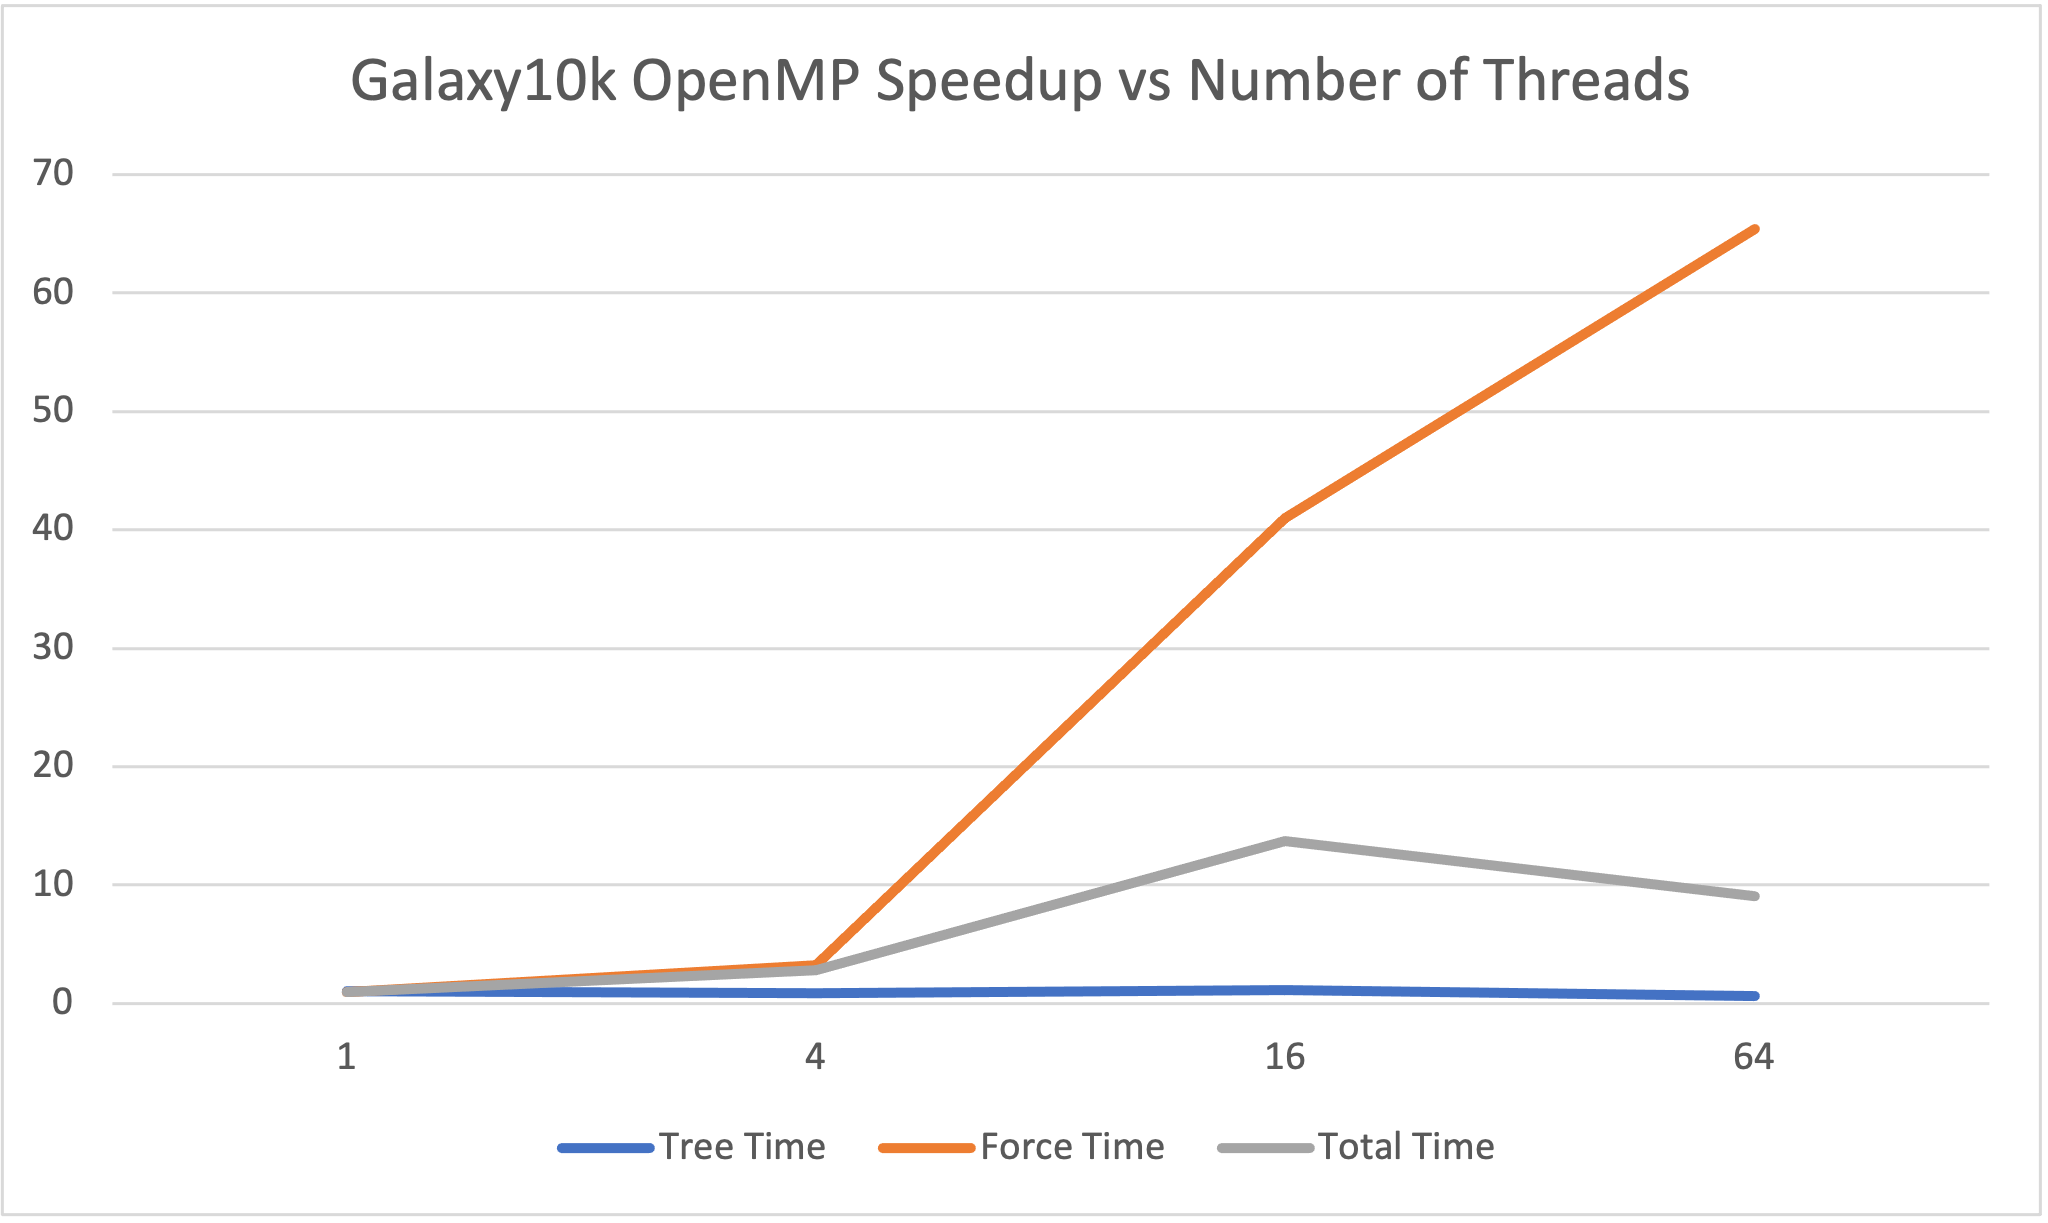
\includegraphics[width=\textwidth]{img/10k_openmp.png}
  \caption{OpenMP Speedup V.S. Number of Threads for Galaxy10K}
  \label{10k_openmp}
\end{figure}
\begin{figure}[h!]
  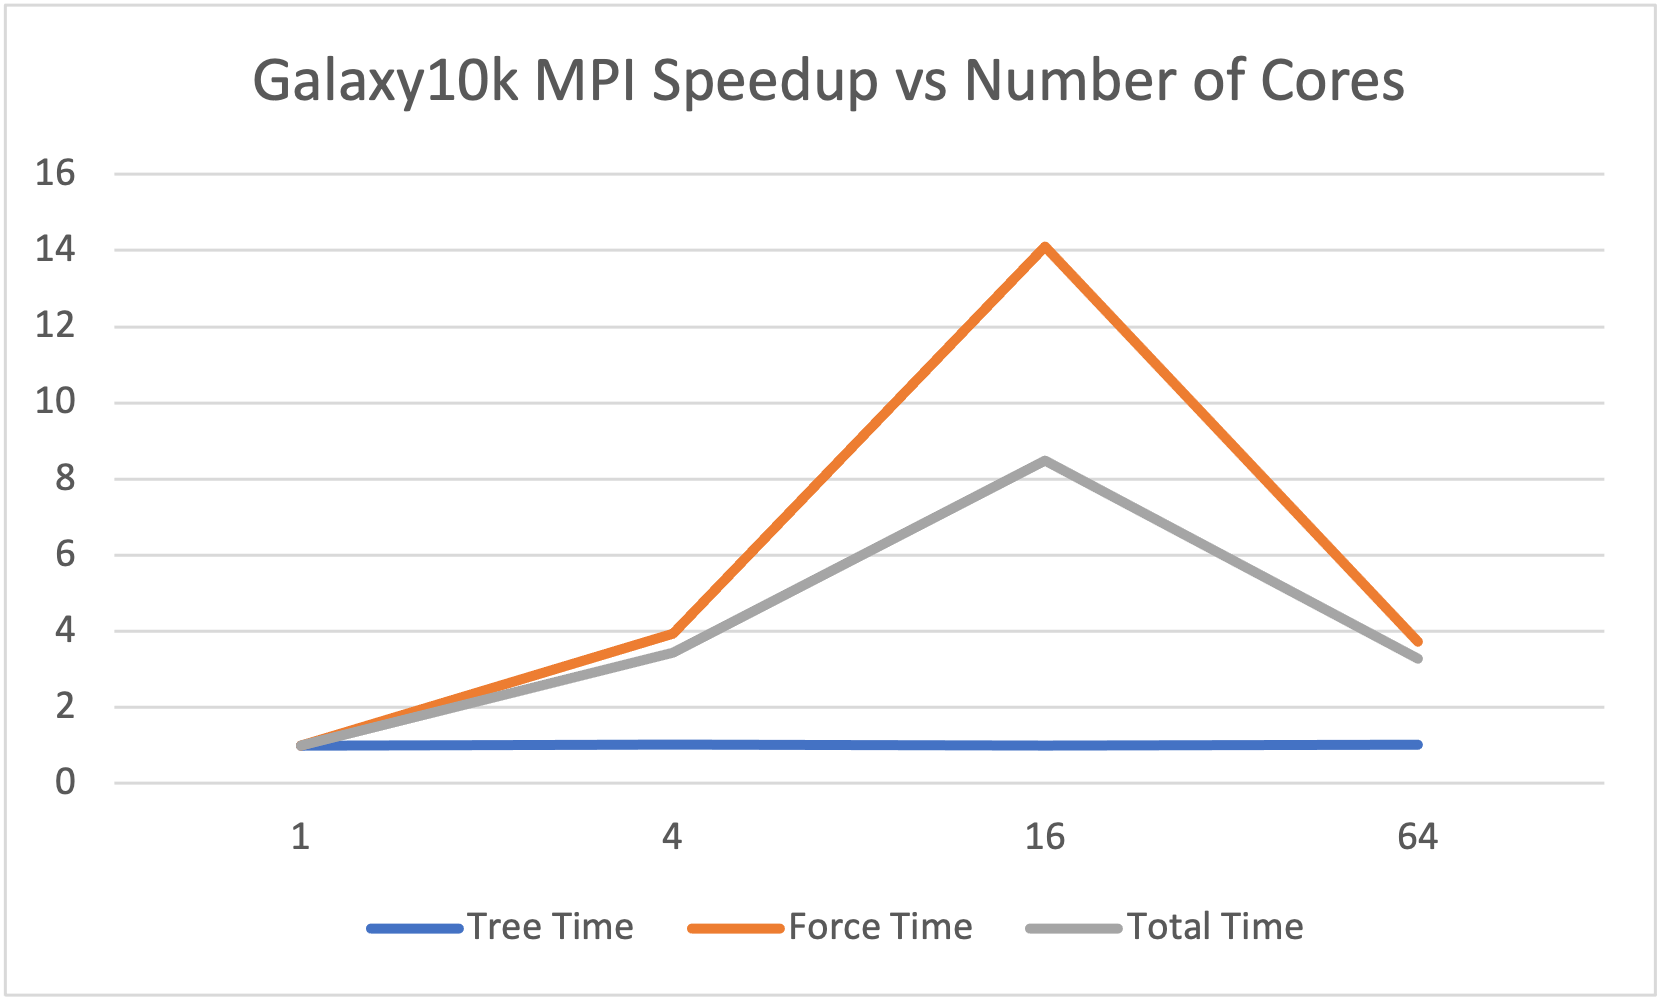
\includegraphics[width=\textwidth]{img/10k_mpi.png}
  \caption{MPI Speedup V.S. Number of Threads for Galaxy10K}
  \label{10k_mpi}
\end{figure}
\begin{figure}[h!]
  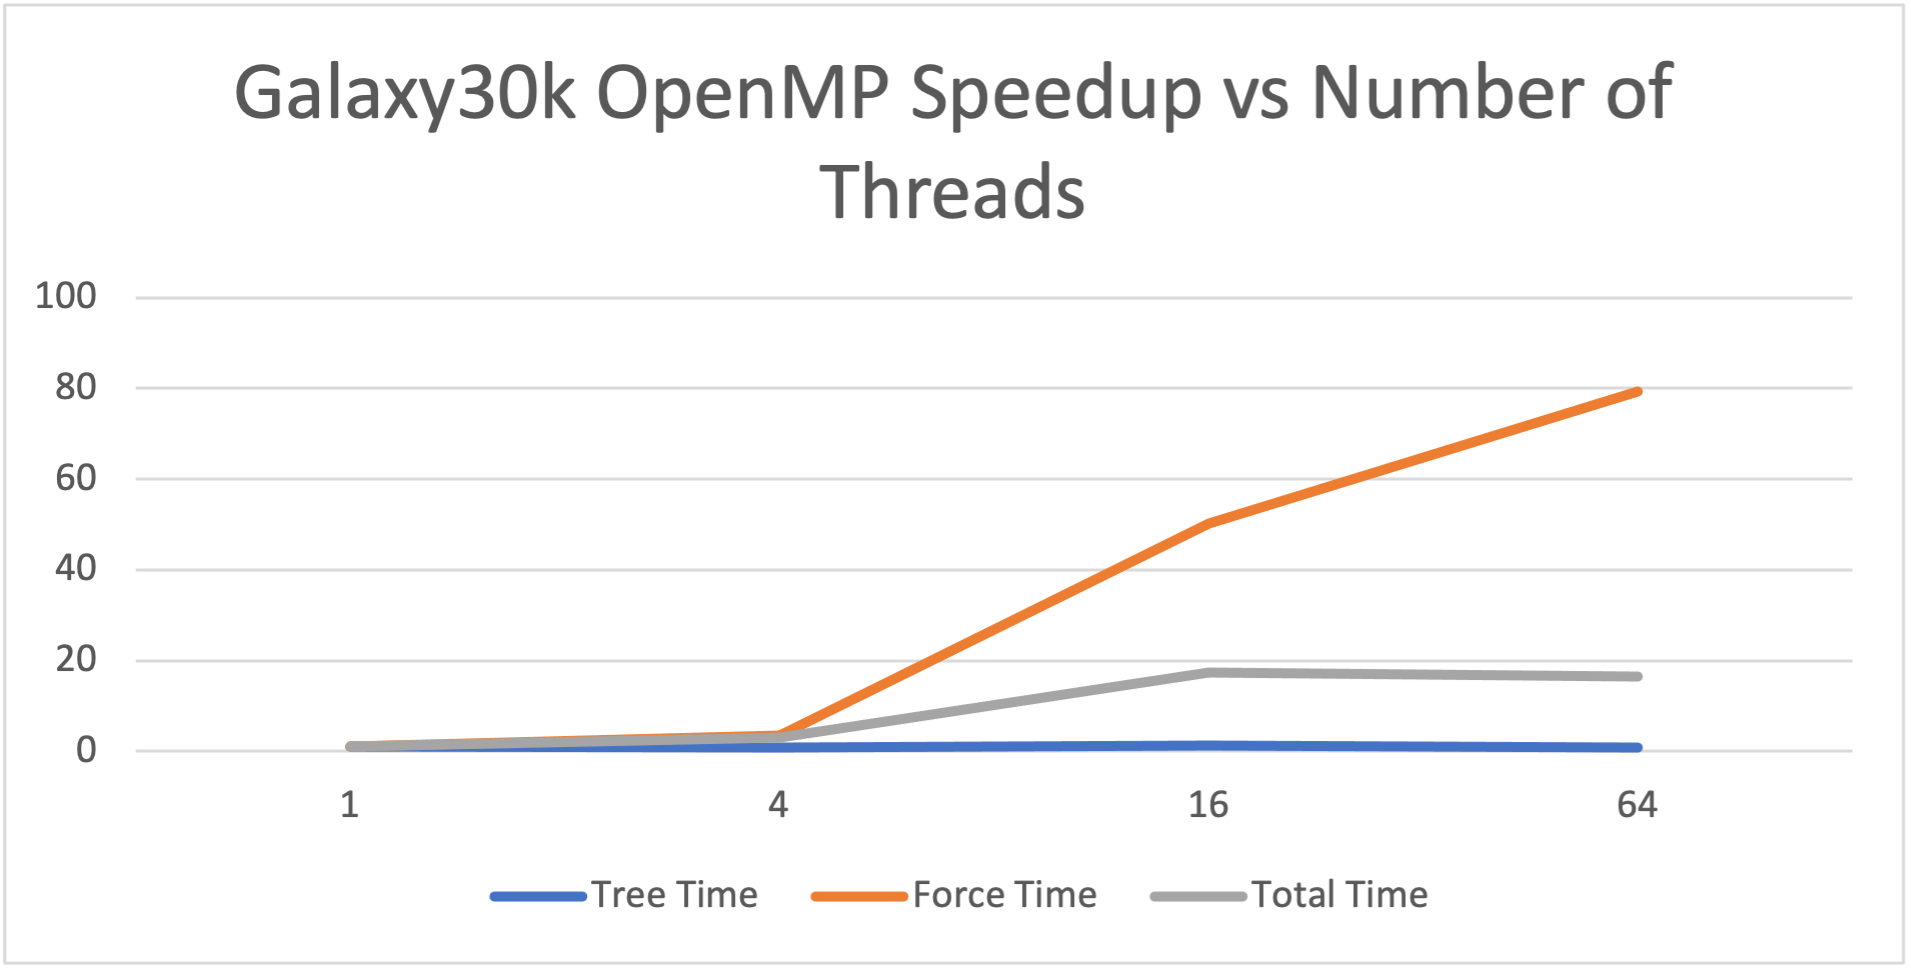
\includegraphics[width=\textwidth]{img/30k_openmp.png}
  \caption{OpenMP Speedup V.S. Number of Threads for Galaxy30K}
  \label{30k_openmp}
\end{figure}
\begin{figure}[h!]
  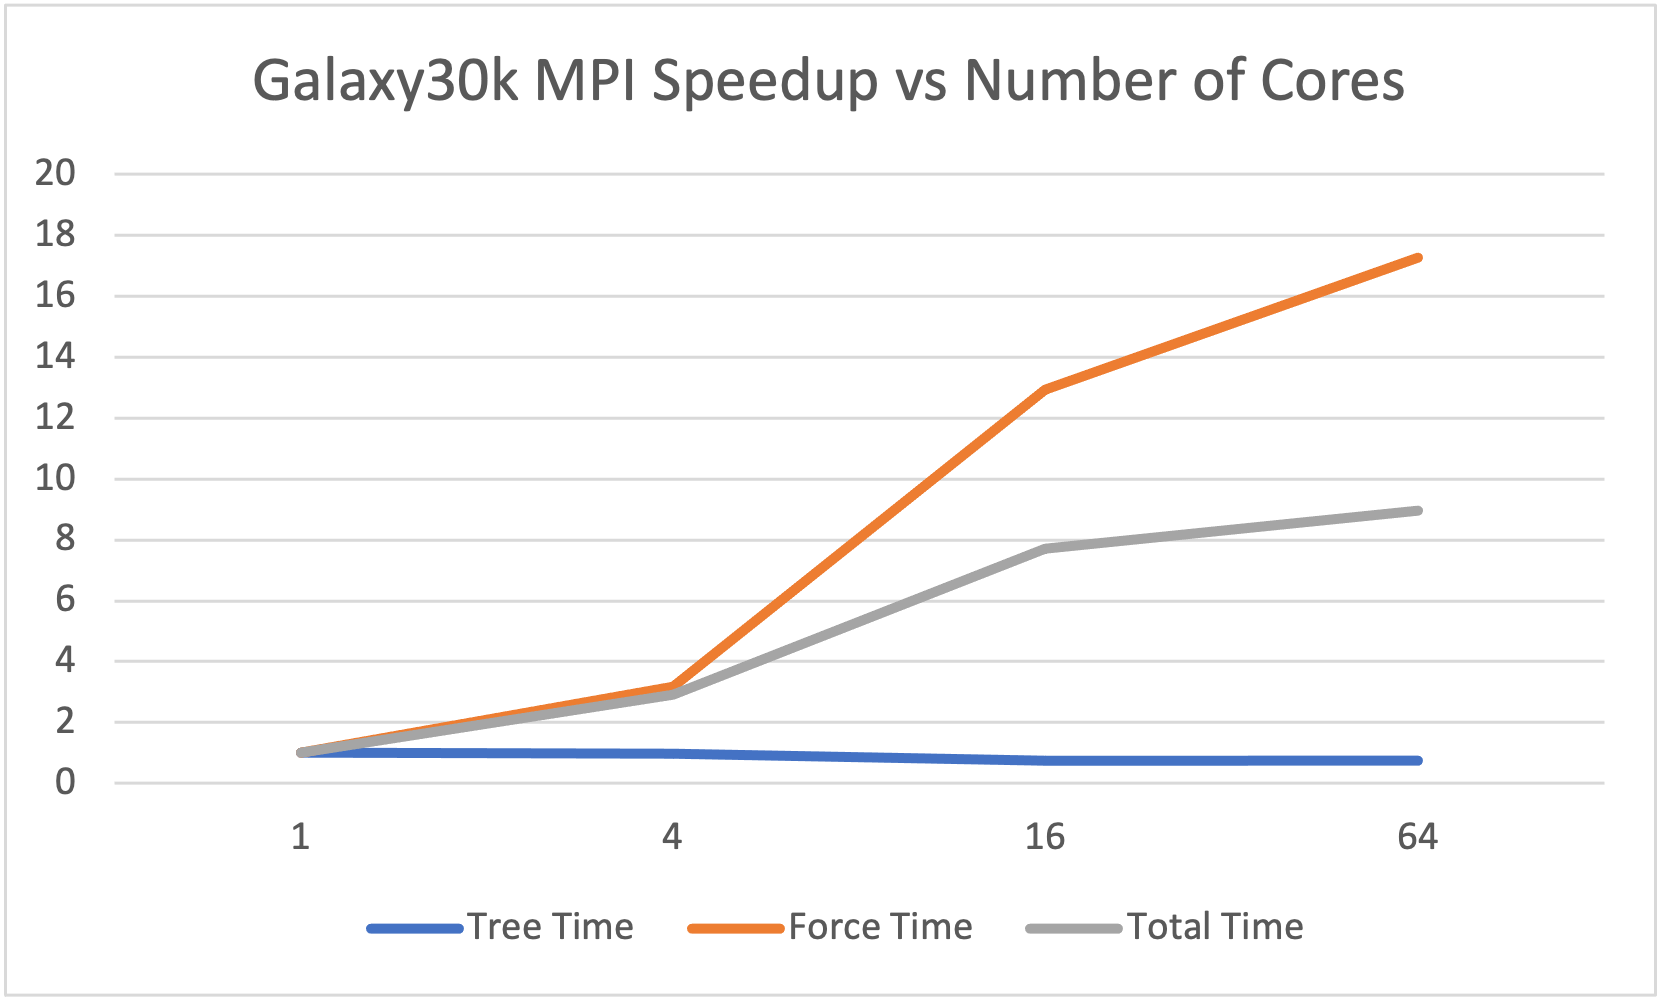
\includegraphics[width=\textwidth]{img/30k_mpi.png}
  \caption{MPI Speedup V.S. Number of Threads for Galaxy30K}
  \label{30k_mpi}
\end{figure}

\subsubsection{Compare different workloads (Galaxy10K V.S. Galaxy30K)}

In this section we examine the performance difference under different problem sizes. From the figures, we can find that the speedup trends as we increase the number of cores/threads are not the same. For Galaxy30k, the speedup always goes up as we increases core number, but for Galaxy10k, the peak speedup is achieved when core number = 16. We think this arises from the small problem size, as the communication-to-computation ratio is large in the Galaxy10k case. We also run experiments on other small input files (2k) and they exhibit similar properties - we don't really gain from the increasing number of cores. 

\subsubsection{Compare different types of metrics (Tree time V.S. Force time V.S. Total Time)}
In this section, we examine the performance difference under different types of metrics, e.g. tree time, force time, and total time. 

In the figures, the tree times represented by the blue lines change little as the number of threads increases. One possible reason is that our parallel tree construction is not efficient enough as we just divide the particles by their positions. The workload distribution is not necessarily even for different threads. Also, dividing and merging the tree incur some overhead and the overhead would increase with more threads. 

The force time represented by the orange lines increase significantly as the number of threads increases which aligns with our expectation except for MPI on Galaxy10K. This increment result from the evenly distributed workload as each thread will receive the same number of particles. 
It could even achieve super-linear speedup when the number of threads increases to 16 or 64. This is because when there are only a few cores, the memory is not large enough to fit in the whole tree and all the particles. As the number of processor increases, the key working set for each thread begins to fit in per-processor cache.

The total time is the sum of tree time and force time, represented by grey line in the figures. In general, the total time changes as the force time changes because when number of threads is small, the force computation is the bottleneck. In a usual single-thread case, the force time is usually 20x of the tree time. However, as the number of threads increases, the speedup for force computation is increases faster than the speedup for tree construction, making tree construction slower than force computation. In our example Galaxy10K, the force time speedup increases while the total time speedup decreases from 16 threads to 64 threads. This is because at this moment, the computation time for force is no longer the bottleneck and tree construction becomes the new bottleneck.

\subsubsection{Compare different parallel models (OpenMP V.S. MPI)}
In this section, we examine the performance difference under different parallel models, OpenMP and MPI. Based on our results, the tree time are roughly the same but OpenMP has better performance in terms of the force time. For OpenMP, each thread is responsible for a different set of particles, and as these particles are stored in the shared global memory, they can directly read and update the particle information. So as the number of threads increases, each thread has fewer particles to compute, so the force time always decreases. For MPI, as the number of threads increases, each core is responsible for fewer particles, however, the communication cost among cores increases as they need to send and receive messages to update the information, which comes free in the OpenMP case. When the workload is large, the reduced computation time outweighs the increased communication time, so we observe an increasing speedup in Galaxy30K case. When the workload is not large enough to exhaust the computation resources, the increased communication time outweighs the reduced computation time, so we observe a turning point in Galaxy10K case.

\subsection{Possible Optimizations}
We have tried to use both the sequential and parallel version of tree construction, but they didn't exhibit a significant difference. One possible reason is that we divide the particles by position, which may not lead to an even distribution of workload. We found the Morton Ordering is one possible solution to construct the QuadTree in parallel, but we failed to figure out how to merge the tree. If we had more time, we would implement the Morton Ordering to achieve greater parallelism in tree construction.

When we implemented the MPI version, instead of constructing the tree in parallel, each node will construct the tree itself before computation. This is because first we didn't find a suitable way to send tree information through MPI, as we define the tree to be recursively represented, and second, the reduced construction time may not be worthy of communication overhead. If the tree construction phase could be parallelized, the performance may be better. 

\section{Work Distribution}
We do all the work together and the credit distribution is 50\% for both Ziyan and Xuanyi.
\begin{itemize}
	\item QuadTree class: Ziyan 50\%, Xuanyi 50\%
	\item Sequential Implementation: Ziyan 50\%, Xuanyi 50\%
	\item OpenMP Implementation: Ziyan 50\%, Xuanyi 50\%
	\item MPI Implementation: Ziyan 50\%, Xuanyi 50\%
\end{itemize}



\bibliographystyle{ieeetr}
{
%\scriptsize
\bibliography{ref}
}


\end{document}
